\documentclass[11pt,a4paper]{article}

\usepackage[utf8]{inputenc}
\usepackage[T1]{fontenc}
\usepackage{mathpazo}
\usepackage[scaled=0.92]{helvet}
\usepackage[margin=1in]{geometry}
\usepackage{graphicx}
\usepackage{amsmath,amssymb,amsfonts}
\usepackage{booktabs}
\usepackage{tabularx}
\usepackage{setspace}
\usepackage{titlesec}
\usepackage{fancyhdr}
\usepackage{float}
\usepackage{caption}
\usepackage{microtype}

\usepackage{tikz}
\usetikzlibrary{shapes.geometric, arrows.meta, positioning, calc, matrix, fit, backgrounds}

\usepackage{listings}
\usepackage{xcolor}
\usepackage[hidelinks]{hyperref}

\setstretch{1.15}
\setlength{\parindent}{0pt}
\setlength{\parskip}{0.8em}
\sloppy

\titleformat{\section}{\normalfont\large\bfseries\sffamily}{\thesection}{1em}{}
\titleformat{\subsection}{\normalfont\normalsize\bfseries\sffamily}{\thesubsection}{1em}{}
\titleformat{\subsubsection}{\normalfont\normalsize\itshape\sffamily}{\thesubsubsection}{1em}{}

\pagestyle{fancy}
\fancyhf{}
\fancyhead[L]{\small\sffamily Fondasi Basis Data: CRUD pada Tingkat Database}
\fancyhead[R]{\small\sffamily\thepage}
\renewcommand{\headrulewidth}{0.4pt}

\captionsetup{font=small,labelfont=bf,labelsep=period}

\renewenvironment{abstract}
{\small
	\begin{center}\textbf{\sffamily Abstrak}\end{center}
	\begin{quote}}
	{\end{quote}}

\lstdefinestyle{code}{
	basicstyle=\ttfamily\small,
	frame=single,
	rulecolor=\color{black},
	breaklines=true,
	showstringspaces=false,
	columns=fullflexible,
	keepspaces=true,
	framesep=6pt,
	aboveskip=1em,
	belowskip=1em,
	xleftmargin=0pt
}

\lstdefinestyle{out}{
	basicstyle=\ttfamily\small,
	frame=tb,
	rulecolor=\color{black},
	breaklines=true,
	showstringspaces=false,
	columns=fullflexible,
	keepspaces=true,
	framesep=4pt,
	aboveskip=1em,
	belowskip=1em
}

\title{\vspace{-1.5cm}\textbf{\sffamily\LARGE Fondasi Basis Data: Menguasai CRUD pada Tingkat Database}}
\author{
	\textbf{Muhammad Riduwan Khafidi} \\
	\small Program Studi Teknik Rekayasa Perangkat Lunak \\
	\small Politeknik Negeri Batam \\
	\small \texttt{4342611034@students.polibatam.ac.id}
}
\date{\small\today}

\begin{document}

\maketitle
\thispagestyle{empty}

\begin{abstract}
	CRUD adalah singkatan dari Create, Read, Update, dan Delete, empat operasi dasar yang membentuk seluruh interaksi dengan sistem penyimpanan data. Namun CRUD tidak berhenti pada baris dan kolom tabel: ia berlapis, dan lapisan paling dasar adalah database itu sendiri. Makalah ini membahas CRUD pada tingkat database secara menyeluruh, mulai dari membangun wadah penyimpanan baru dengan \texttt{CREATE DATABASE}, menelusuri katalog dengan \texttt{SHOW DATABASES} dan \texttt{USE}, mengubah karakteristik wadah dengan \texttt{ALTER DATABASE}, hingga menghapusnya dengan \texttt{DROP DATABASE} beserta segala konsekuensinya. Setiap perintah dilengkapi diagram alur, simulasi keluaran, dan skenario kegagalan yang lazim terjadi. Makalah ini menjadi fondasi sebelum pembaca melangkah ke CRUD pada tingkat tabel dan baris.
\end{abstract}

\section{Pendahuluan: Mengapa Database Punya Lapisan}

\subsection{Analogi Sistem Berkas}

Sebuah komputer menata berkasnya dalam hierarki. Di puncak ada sistem berkas, di bawahnya ada folder, dan di dalam folder ada berkas. Basis data meniru struktur itu.

\begin{figure}[H]
	\centering
	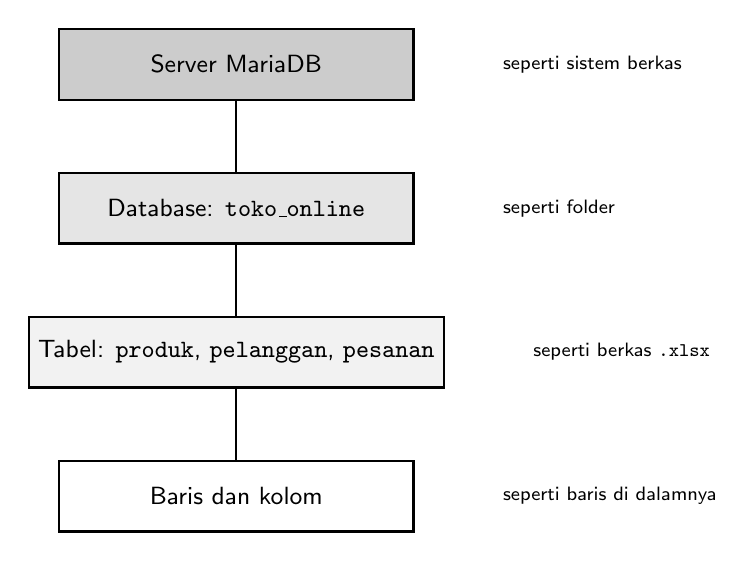
\begin{tikzpicture}[
			node distance=0.6cm and 0.8cm,
			lvl/.style={rectangle, draw=black, thick, minimum width=4.5cm, minimum height=0.9cm, align=center, font=\sffamily\small},
			line/.style={draw, thick}
		]
		\node[lvl, fill=black!20] (server) {Server MariaDB};
		\node[lvl, fill=black!10, below=0.9cm of server] (db) {Database: \texttt{toko\_online}};
		\node[lvl, fill=black!5, below=0.9cm of db] (table) {Tabel: \texttt{produk}, \texttt{pelanggan}, \texttt{pesanan}};
		\node[lvl, fill=white, below=0.9cm of table] (row) {Baris dan kolom};

		\draw[line] (server) -- (db);
		\draw[line] (db) -- (table);
		\draw[line] (table) -- (row);

		\node[font=\scriptsize\sffamily, right=1cm of server] {seperti sistem berkas};
		\node[font=\scriptsize\sffamily, right=1cm of db] {seperti folder};
		\node[font=\scriptsize\sffamily, right=1cm of table] {seperti berkas \texttt{.xlsx}};
		\node[font=\scriptsize\sffamily, right=1cm of row] {seperti baris di dalamnya};
	\end{tikzpicture}
	\caption{Hierarki server, database, tabel, dan baris sebagai analogi sistem berkas.}
	\label{fig:hierarchy}
\end{figure}

Pada makalah sebelumnya dibahas tipe data di tingkat kolom. Makalah ini naik satu lapis ke atas dan membahas wadah di mana seluruh kolom itu tinggal: database. Tanpa database yang dibuat dengan benar, tabel tidak punya tempat untuk hidup. Tanpa pemahaman cara menghapusnya dengan aman, satu perintah \texttt{DROP} bisa menghilangkan data setahun.

\subsection{Empat Operasi, Satu Siklus Hidup}

CRUD pada tingkat database membentuk satu siklus hidup yang utuh, seperti pada Gambar~\ref{fig:crud-cycle}.

\begin{figure}[H]
	\centering
	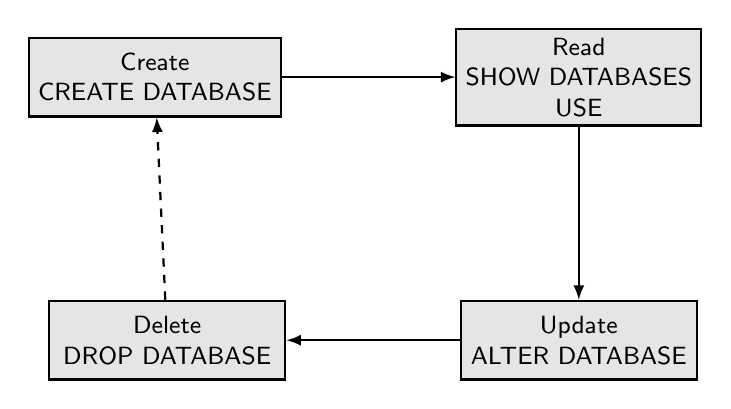
\begin{tikzpicture}[
			node distance=2.2cm,
			op/.style={rectangle, draw=black, thick, fill=black!10, minimum width=3cm, minimum height=1cm, align=center, font=\sffamily\small},
			cmd/.style={font=\ttfamily\scriptsize},
			line/.style={draw, thick, -latex}
		]
		\node[op] (create) {Create \\ \cmd{CREATE DATABASE}};
		\node[op, right=of create] (read) {Read \\ \cmd{SHOW DATABASES} \\ \cmd{USE}};
		\node[op, below=of read] (update) {Update \\ \cmd{ALTER DATABASE}};
		\node[op, left=of update] (delete) {Delete \\ \cmd{DROP DATABASE}};

		\draw[line] (create) -- (read);
		\draw[line] (read) -- (update);
		\draw[line] (update) -- (delete);
		\draw[line, dashed] (delete) -- (create);
	\end{tikzpicture}
	\caption{Siklus hidup CRUD pada tingkat database.}
	\label{fig:crud-cycle}
\end{figure}

Garis putus-putus dari \texttt{DROP} kembali ke \texttt{CREATE} menandakan bahwa setelah database dihapus, biasanya akan dibuat database baru sebagai pengganti, misalnya saat migrasi atau pengujian.

\section{Menyiapkan Konteks: Masuk ke Server}

Sebelum semua perintah CRUD database bisa dijalankan, kita harus berada di dalam server MariaDB. Di terminal Linux, masuk melalui klien \texttt{mariadb} atau \texttt{mycli}.

\begin{lstlisting}[style=code]
mariadb -u root -p
\end{lstlisting}

Setelah memasukkan kata sandi, prompt berubah menjadi seperti berikut.

\begin{lstlisting}[style=out]
MariaDB [(none)]>
\end{lstlisting}

Kurung siku berisi \texttt{none} menandakan belum ada database yang dipilih. Prompt inilah tempat seluruh perintah pada makalah ini diketik.

\section{Create: Membangun Wadah Baru}

\subsection{Sintaks Dasar}

Perintah \texttt{CREATE DATABASE} memiliki dua bentuk yang setara. \texttt{SCHEMA} adalah sinonim dari \texttt{DATABASE} di MariaDB dan MySQL, warisan dari standar SQL.

\begin{lstlisting}[style=code]
CREATE DATABASE nama_database;
CREATE SCHEMA nama_database;
\end{lstlisting}

Kedua baris menghasilkan efek yang persis sama. Konvensi yang lazim dipakai adalah \texttt{DATABASE}, sedangkan \texttt{SCHEMA} muncul lebih sering di lingkungan PostgreSQL.

\subsection{Varian Lengkap}

Selain bentuk dasar, \texttt{CREATE DATABASE} menerima beberapa klausa opsional yang penting untuk produksi.

\begin{lstlisting}[style=code]
CREATE DATABASE [IF NOT EXISTS] nama_database
    [CHARACTER SET nama_charset]
    [COLLATE nama_collation]
    [COMMENT 'teks keterangan'];
\end{lstlisting}

Setiap klausa punya peran yang berbeda, seperti dijelaskan pada Tabel~\ref{tab:create-clauses}.

\begin{table}[H]
	\centering
	\caption{Klausa opsional pada \texttt{CREATE DATABASE}.}
	\label{tab:create-clauses}
	\small
	\begin{tabularx}{\textwidth}{l X}
		\toprule
		Klausa                 & Fungsi                                                                \\
		\midrule
		\texttt{IF NOT EXISTS} & Mencegah error jika database dengan nama sama sudah ada.              \\
		\texttt{CHARACTER SET} & Menentukan pengodean karakter bawaan untuk seluruh tabel di dalamnya. \\
		\texttt{COLLATE}       & Menentukan aturan pembandingan dan pengurutan teks.                   \\
		\texttt{COMMENT}       & Menyimpan catatan dokumentasi pada katalog.                           \\
		\bottomrule
	\end{tabularx}
\end{table}

\subsection{Contoh Nyata dan Keluarannya}

\begin{lstlisting}[style=code]
CREATE DATABASE toko_online
    CHARACTER SET utf8mb4
    COLLATE utf8mb4_unicode_ci
    COMMENT 'Database produksi toko online';
\end{lstlisting}

Jika berhasil, MariaDB menampilkan konfirmasi singkat.

\begin{lstlisting}[style=out]
Query OK, 1 row affected
\end{lstlisting}

Jika diulang tanpa \texttt{IF NOT EXISTS}, MariaDB menolak.

\begin{lstlisting}[style=out]
ERROR 1007 (HY000): Can't create database 'toko_online';
database exists
\end{lstlisting}

Dengan \texttt{IF NOT EXISTS}, pengulangan tidak menghasilkan error, hanya peringatan halus.

\begin{lstlisting}[style=code]
CREATE DATABASE IF NOT EXISTS toko_online;
\end{lstlisting}

\begin{lstlisting}[style=out]
Query OK, 1 row affected, 1 warning
\end{lstlisting}

\subsection{Alur Keputusan Sebelum Membuat Database}

Membuat database bukan sekadar mengetik perintah. Ada beberapa pertanyaan yang sebaiknya dijawab lebih dulu, seperti pada Gambar~\ref{fig:create-flow}.

\begin{figure}[H]
	\centering
	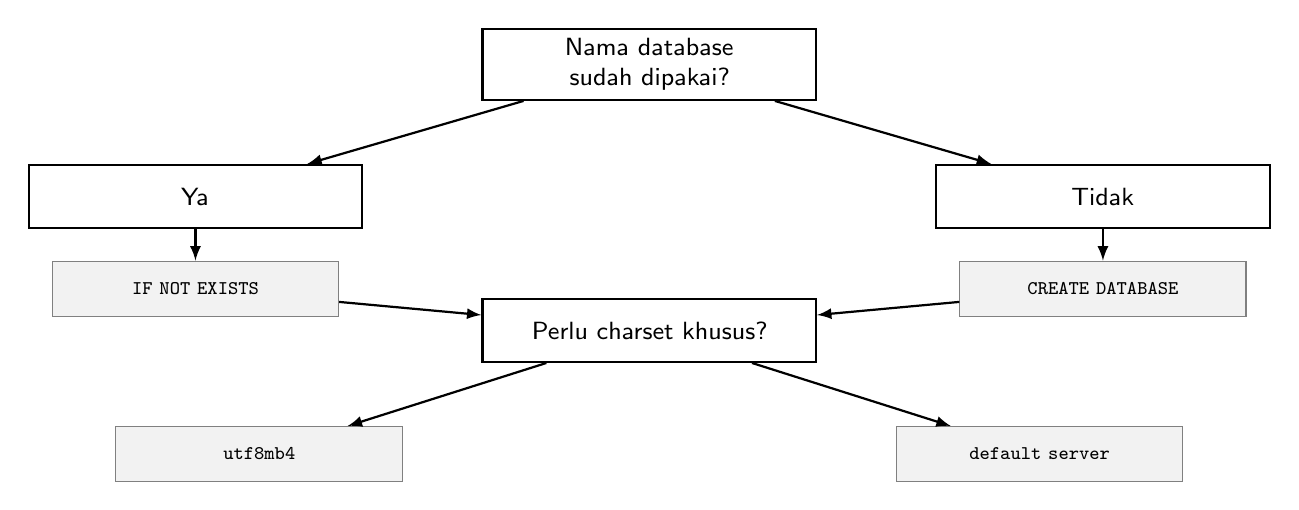
\begin{tikzpicture}[
			node distance=0.5cm and 1cm,
			q/.style={rectangle, draw=black, thick, fill=white, text width=4cm, align=center, minimum height=0.8cm, font=\sffamily\small},
			a/.style={rectangle, draw=black!50, fill=black!5, text width=3.4cm, align=center, minimum height=0.7cm, font=\ttfamily\scriptsize},
			line/.style={draw, thick, -latex}
		]
		\node[q] (start) {Nama database sudah dipakai?};
		\node[q, below left=0.8cm and 1.5cm of start] (yes) {Ya};
		\node[q, below right=0.8cm and 1.5cm of start] (no) {Tidak};
		\node[a, below=0.4cm of yes] (y1) {\texttt{IF NOT EXISTS}};
		\node[a, below=0.4cm of no] (n1) {\texttt{CREATE DATABASE}};

		\node[q, below=2.5cm of start] (charset) {Perlu charset khusus?};
		\node[a, below left=0.8cm and 1cm of charset] (c1) {\texttt{utf8mb4}};
		\node[a, below right=0.8cm and 1cm of charset] (c2) {default server};

		\draw[line] (start) -- (yes);
		\draw[line] (start) -- (no);
		\draw[line] (yes) -- (y1);
		\draw[line] (no) -- (n1);
		\draw[line] (y1) -- (charset);
		\draw[line] (n1) -- (charset);
		\draw[line] (charset) -- (c1);
		\draw[line] (charset) -- (c2);
	\end{tikzpicture}
	\caption{Alur keputusan sebelum menjalankan \texttt{CREATE DATABASE}.}
	\label{fig:create-flow}
\end{figure}

\subsection{Mengapa \texttt{utf8mb4} dan Bukan \texttt{utf8}}

MariaDB memiliki dua charset yang namanya mirip tetapi berperilaku berbeda. \texttt{utf8} di MariaDB hanyalah alias untuk \texttt{utf8mb3}, yang hanya mendukung karakter hingga tiga byte. Emoji dan beberapa aksara Asia membutuhkan empat byte. Jika Anda membuat database dengan \texttt{utf8} lalu mencoba menyimpan emoji, karakter tersebut akan terpotong atau ditolak.

\texttt{utf8mb4} mendukung seluruh rentang Unicode, termasuk emoji. Untuk database baru pada tahun 2020 ke atas, \texttt{utf8mb4} adalah pilihan bawaan yang tepat. Collation yang umum dipakai adalah \texttt{utf8mb4\_unicode\_ci}, dengan \texttt{ci} berarti \textit{case-insensitive}, sehingga pembandingan tidak membedakan huruf besar dan kecil.

\section{Read: Menelusuri Katalog Database}

Operasi Read pada tingkat database terdiri dari dua perintah yang saling melengkapi: melihat daftar seluruh database, dan memilih salah satu untuk dijadikan konteks kerja.

\subsection{Melihat Seluruh Database}

\begin{lstlisting}[style=code]
SHOW DATABASES;
\end{lstlisting}

Keluaran perintah ini berupa tabel satu kolom.

\begin{lstlisting}[style=out]
+--------------------+
| Database           |
+--------------------+
| information_schema |
| mysql              |
| performance_schema |
| sys                |
| toko_online        |
+--------------------+
5 rows in set (0.001 sec)
\end{lstlisting}

Empat baris pertama adalah database sistem yang dibuat otomatis oleh MariaDB saat instalasi. Penjelasannya ada pada Tabel~\ref{tab:sys-db}.

\begin{table}[H]
	\centering
	\caption{Database sistem bawaan MariaDB.}
	\label{tab:sys-db}
	\small
	\begin{tabularx}{\textwidth}{l X}
		\toprule
		Database                     & Isi                                                          \\
		\midrule
		\texttt{information\_schema} & Katalog metadata tentang seluruh database, tabel, dan kolom. \\
		\texttt{mysql}               & Tabel pengguna, hak akses, dan konfigurasi server.           \\
		\texttt{performance\_schema} & Statistik kinerja dan profil eksekusi query.                 \\
		\texttt{sys}                 & Tampilan ringkas dari \texttt{performance\_schema}.          \\
		\bottomrule
	\end{tabularx}
\end{table}

\texttt{information\_schema} adalah database khusus yang tidak menyimpan data pengguna, melainkan metadata. Isinya dihasilkan langsung oleh server setiap kali di-query, sehingga tidak bisa di-\texttt{DROP} atau di-\texttt{UPDATE} secara langsung.

\subsection{Varian Filter}

\texttt{SHOW DATABASES} juga menerima klausa \texttt{LIKE} untuk menyaring hasil berdasarkan pola.

\begin{lstlisting}[style=code]
SHOW DATABASES LIKE 'toko%';
SHOW DATABASES WHERE \`Database\` = 'toko_online';
\end{lstlisting}

Keluaran pertama hanya menampilkan database yang namanya diawali \texttt{toko}. Tanda persen berperan sebagai wildcard, sama seperti pada \texttt{LIKE} di SQL umumnya.

\subsection{Memilih Database Aktif}

Setelah tahu nama database, langkah berikutnya adalah masuk ke dalamnya dengan \texttt{USE}.

\begin{lstlisting}[style=code]
USE toko_online;
\end{lstlisting}

\begin{lstlisting}[style=out]
Database changed
\end{lstlisting}

Prompt langsung berubah menandakan konteks kerja sudah berpindah.

\begin{lstlisting}[style=out]
MariaDB [toko_online]>
\end{lstlisting}

Setelah \texttt{USE}, semua perintah tabel seperti \texttt{CREATE TABLE}, \texttt{SELECT}, dan \texttt{DROP TABLE} akan berlaku pada database \texttt{toko\_online} tanpa perlu menyebut nama database setiap kali.

Jika nama database salah, MariaDB menolak.

\begin{lstlisting}[style=out]
ERROR 1049 (42000): Unknown database 'toko_onlinee'
\end{lstlisting}

Untuk memeriksa database mana yang sedang aktif tanpa melihat prompt, gunakan fungsi \texttt{DATABASE()}.

\begin{lstlisting}[style=code]
SELECT DATABASE();
\end{lstlisting}

\begin{lstlisting}[style=out]
+--------------+
| DATABASE()   |
+--------------+
| toko_online  |
+--------------+
\end{lstlisting}

\subsection{Diagram Perpindahan Konteks}

Gambar~\ref{fig:use-context} mengilustrasikan bagaimana \texttt{USE} memindahkan konteks kerja tanpa mengubah data apa pun.

\begin{figure}[H]
	\centering
	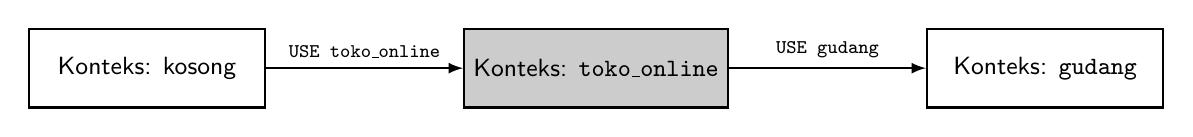
\begin{tikzpicture}[
			nd/.style={rectangle, draw=black, thick, fill=white, minimum width=3cm, minimum height=1cm, align=center, font=\sffamily\small},
			act/.style={rectangle, draw=black, thick, fill=black!20, minimum width=3cm, minimum height=1cm, align=center, font=\sffamily\small},
			line/.style={draw, thick, -latex}
		]
		\node[nd] (none) {Konteks: kosong};
		\node[act, right=2.5cm of none] (one) {Konteks: \texttt{toko\_online}};
		\node[nd, right=2.5cm of one] (two) {Konteks: \texttt{gudang}};

		\draw[line] (none) -- node[above, font=\scriptsize\sffamily] {\texttt{USE toko\_online}} (one);
		\draw[line] (one) -- node[above, font=\scriptsize\sffamily] {\texttt{USE gudang}} (two);
	\end{tikzpicture}
	\caption{Perpindahan konteks kerja dengan \texttt{USE}.}
	\label{fig:use-context}
\end{figure}

Perpindahan konteks bersifat sementara. Jika sesi ditutup lalu dibuka kembali, konteks kembali kosong dan \texttt{USE} harus dijalankan ulang.

\section{Update: Mengubah Karakteristik Database}

Pada tingkat database, operasi Update tidak mengubah data baris (itu tugas \texttt{UPDATE} di tingkat tabel), melainkan mengubah karakteristik wadah: charset, collation, dan pada beberapa mesin basis data, mode baca-saja.

\subsection{Sintaks Dasar}

\begin{lstlisting}[style=code]
ALTER DATABASE nama_database
    [CHARACTER SET nama_charset]
    [COLLATE nama_collation];
\end{lstlisting}

\texttt{ALTER SCHEMA} adalah sinonim yang setara.

\subsection{Mengubah Charset dan Collation}

Misalnya sebuah database lama dibuat dengan charset bawaan yang keliru. Charset-nya bisa diperbaiki.

\begin{lstlisting}[style=code]
ALTER DATABASE toko_online
    CHARACTER SET utf8mb4
    COLLATE utf8mb4_unicode_ci;
\end{lstlisting}

\begin{lstlisting}[style=out]
Query OK, 1 row affected
\end{lstlisting}

Penting dipahami: \texttt{ALTER DATABASE} hanya mengubah pengaturan bawaan. Tabel yang sudah ada sebelumnya tidak ikut berubah charset-nya. Untuk mengubah tabel dan kolom yang sudah ada, perlu \texttt{ALTER TABLE} terpisah per tabel, atau konversi bertahap.

\subsection{Apa yang Tidak Bisa Dilakukan}

Banyak pemula mencoba \texttt{RENAME DATABASE} dan terkejut karena perintah itu tidak ada.

\begin{lstlisting}[style=code]
RENAME DATABASE toko_online TO toko_baru;
\end{lstlisting}

\begin{lstlisting}[style=out]
ERROR 1064 (42000): You have an error in your SQL syntax;
check the manual that corresponds to your MariaDB server
version for the right syntax to use near
'DATABASE toko_online TO toko_baru' at line 1
\end{lstlisting}

MariaDB dan MySQL memang tidak menyediakan perintah \texttt{RENAME DATABASE}. Ada dua alasan historis. Pertama, operasi ini berisiko jika ada tabel yang sedang dibuka oleh sesi lain. Kedua, dalam sistem terdistribusi, mengganti nama database bisa mematahkan replikasi.

Sebagai gantinya, ada tiga jalur resmi seperti pada Tabel~\ref{tab:rename-alt}.

\begin{table}[H]
	\centering
	\caption{Alternatif saat ingin mengganti nama database.}
	\label{tab:rename-alt}
	\small
	\begin{tabularx}{\textwidth}{l X}
		\toprule
		Pendekatan       & Langkah singkat                                                                                      \\
		\midrule
		Dump dan restore & \texttt{mysqldump} database lama, buat database baru, restore ke sana, lalu \texttt{DROP} yang lama. \\
		Pindahkan tabel  & Buat database baru, gunakan \texttt{RENAME TABLE lama.t TO baru.t} untuk setiap tabel.               \\
		Simpan tautan    & Buat \texttt{VIEW} atau nama alias di aplikasi tanpa mengubah struktur.                              \\
		\bottomrule
	\end{tabularx}
\end{table}

\subsection{Alur Update Database}

Gambar~\ref{fig:alter-flow} merangkum kapan \texttt{ALTER DATABASE} berguna dan kapan harus memakai pendekatan lain.

\begin{figure}[H]
	\centering
	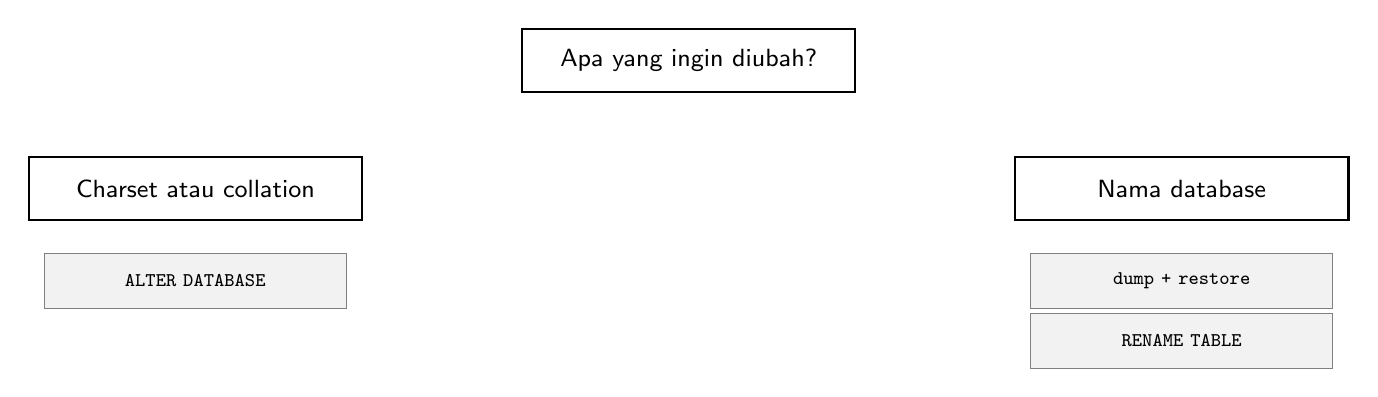
\begin{tikzpicture}[
			node distance=0.6cm and 1cm,
			q/.style={rectangle, draw=black, thick, fill=white, text width=4cm, align=center, minimum height=0.8cm, font=\sffamily\small},
			a/.style={rectangle, draw=black!50, fill=black!5, text width=3.6cm, align=center, minimum height=0.7cm, font=\ttfamily\scriptsize},
			line/.style={draw, thick, -latex}
		]
		\node[q] (start) {Apa yang ingin diubah?};
		\node[q, below left=0.8cm and 2cm of start] (cs) {Charset atau collation};
		\node[q, below right=0.8cm and 2cm of start] (nm) {Nama database};

		\node[a, below=0.4cm of cs] (cs1) {\texttt{ALTER DATABASE}};
		\node[a, below=0.4cm of nm] (nm1) {dump + restore};
		\node[a, below=0.05cm of nm1] (nm2) {\texttt{RENAME TABLE}};
	\end{tikzpicture}
	\caption{Alur memilih operasi update pada tingkat database.}
	\label{fig:alter-flow}
\end{figure}

\subsection{Memeriksa Hasil Perubahan}

Setelah \texttt{ALTER DATABASE}, hasilnya bisa diperiksa dengan \texttt{SHOW CREATE DATABASE}.

\begin{lstlisting}[style=code]
SHOW CREATE DATABASE toko_online;
\end{lstlisting}

\begin{lstlisting}[style=out]
+-------------+-----------------------------------------------------+
| Database    | Create Database                                     |
+-------------+-----------------------------------------------------+
| toko_online | CREATE DATABASE `toko_online`
                /*!40100 DEFAULT CHARACTER SET utf8mb4
                COLLATE utf8mb4_unicode_ci */
                /*!80016 COMMENT 'Database produksi toko online' */ |
+-------------+-----------------------------------------------------+
\end{lstlisting}

Keluaran ini menampilkan perintah \texttt{CREATE DATABASE} yang persis akan dijalankan jika database dibuat ulang dari nol. Ini cara paling andal untuk memverifikasi charset, collation, dan komentar yang sedang aktif.

\section{Delete: Menghapus Database}

\subsection{Sintaks Dasar}

\begin{lstlisting}[style=code]
DROP DATABASE [IF EXISTS] nama_database;
\end{lstlisting}

Perintah ini menghapus seluruh database beserta semua tabel, indeks, view, trigger, dan data di dalamnya. Tidak ada tombol undo. Tidak ada tempat sampah. Tidak ada konfirmasi.

\begin{lstlisting}[style=code]
DROP DATABASE toko_online;
\end{lstlisting}

\begin{lstlisting}[style=out]
Query OK, 0 rows affected
\end{lstlisting}

Keluaran \texttt{0 rows affected} bisa menyesatkan. Angka nol itu merujuk pada baris data, bukan pada ada atau tidaknya database. Database tetap terhapus, terlepas dari berapa banyak tabel di dalamnya.

\subsection{\texttt{IF EXISTS} dan Perilakunya}

Tanpa \texttt{IF EXISTS}, menghapus database yang tidak ada akan menghasilkan error.

\begin{lstlisting}[style=out]
ERROR 1008 (HY000): Can't drop database 'toko_online';
database doesn't exist
\end{lstlisting}

Dengan \texttt{IF EXISTS}, penghapusan yang gagal tidak dianggap error.

\begin{lstlisting}[style=code]
DROP DATABASE IF EXISTS toko_online;
\end{lstlisting}

\begin{lstlisting}[style=out]
Query OK, 0 rows affected, 1 warning
\end{lstlisting}

\texttt{IF EXISTS} sering dipakai di skrip migrasi atau pengujian yang dijalankan berulang, karena hasilnya selalu sukses tanpa perlu mengecek keberadaan database lebih dulu.

\subsection{Konsekuensi Berantai}

Gambar~\ref{fig:drop-cascade} menunjukkan bagaimana satu perintah \texttt{DROP DATABASE} menghapus semua lapisan di bawahnya secara berantai.

\begin{figure}[H]
	\centering
	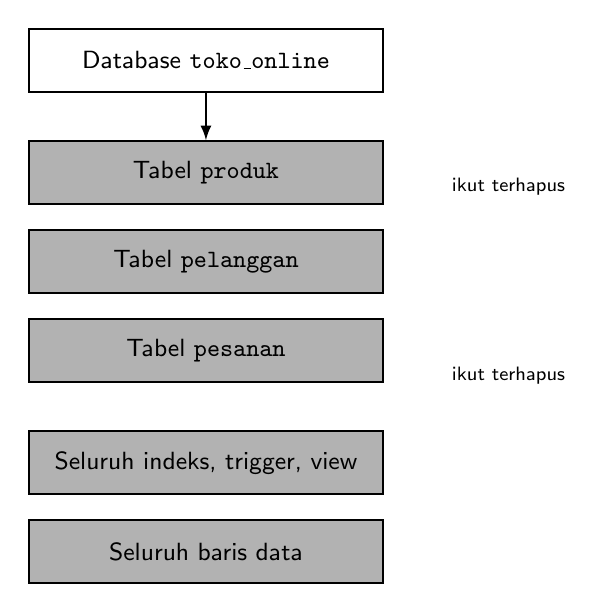
\begin{tikzpicture}[
			node distance=0.6cm and 0.8cm,
			lvl/.style={rectangle, draw=black, thick, minimum width=4.5cm, minimum height=0.8cm, align=center, font=\sffamily\small},
			gone/.style={rectangle, draw=black, thick, fill=black!30, minimum width=4.5cm, minimum height=0.8cm, align=center, font=\sffamily\small},
			line/.style={draw, thick, -latex}
		]
		\node[lvl, fill=white] (db) {Database \texttt{toko\_online}};
		\node[gone, below=0.6cm of db] (t1) {Tabel \texttt{produk}};
		\node[gone, below=0.3cm of t1] (t2) {Tabel \texttt{pelanggan}};
		\node[gone, below=0.3cm of t2] (t3) {Tabel \texttt{pesanan}};
		\node[gone, below=0.6cm of t3] (idx) {Seluruh indeks, trigger, view};
		\node[gone, below=0.3cm of idx] (data) {Seluruh baris data};

		\draw[line] (db) -- (t1);
		\node[font=\scriptsize\sffamily, anchor=west] at (3, -1.6) {ikut terhapus};
		\node[font=\scriptsize\sffamily, anchor=west] at (3, -4.0) {ikut terhapus};
	\end{tikzpicture}
	\caption{Konsekuensi berantai satu perintah \texttt{DROP DATABASE}.}
	\label{fig:drop-cascade}
\end{figure}

\subsection{Prosedur Aman Sebelum \texttt{DROP}}

Penghapusan database yang tidak disengaja adalah salah satu insiden paling sering dilaporkan di forum basis data. Gambar~\ref{fig:drop-safe} menyajikan prosedur minimal yang sebaiknya dilalui.

\begin{figure}[H]
	\centering
	\begin{tikzpicture}[
			node distance=0.5cm,
			step/.style={rectangle, draw=black, thick, fill=black!5, text width=9cm, align=left, minimum height=0.8cm, font=\sffamily\small, inner sep=8pt},
			line/.style={draw, thick, -latex}
		]
		\node[step] (s1) {\textbf{1.} Pastikan sesi tidak sedang memakai database: \texttt{SELECT DATABASE();}};
		\node[step, below=0.4cm of s1] (s2) {\textbf{2.} Buat cadangan: \texttt{mysqldump -u root -p toko\_online > backup.sql}};
		\node[step, below=0.4cm of s2] (s3) {\textbf{3.} Verifikasi berkas cadangan: \texttt{ls -lh backup.sql}};
		\node[step, below=0.4cm of s3] (s4) {\textbf{4.} Uji restore di server sementara jika waktu memungkinkan};
		\node[step, below=0.4cm of s4] (s5) {\textbf{5.} Baru jalankan \texttt{DROP DATABASE toko\_online;}};

		\draw[line] (s1) -- (s2);
		\draw[line] (s2) -- (s3);
		\draw[line] (s3) -- (s4);
		\draw[line] (s4) -- (s5);
	\end{tikzpicture}
	\caption{Prosedur aman sebelum menghapus database.}
	\label{fig:drop-safe}
\end{figure}

Perintah cadangan pada langkah kedua adalah penyelamat utama. Berkas \texttt{backup.sql} bisa dipulihkan dengan satu perintah.

\begin{lstlisting}[style=code]
mariadb -u root -p toko_online < backup.sql
\end{lstlisting}

Selama berkas cadangan ada, penghapusan database tidak lagi bersifat final.

\subsection{Menghapus Banyak Database Sekaligus}

MariaDB tidak memiliki sintaks \texttt{DROP DATABASE db1, db2, db3}. Untuk menghapus beberapa database, perintah harus dijalankan berulang. Pada skrip, ini biasanya dilakukan dalam satu sesi.

\begin{lstlisting}[style=code]
DROP DATABASE IF EXISTS db_lama;
DROP DATABASE IF EXISTS db_uji;
DROP DATABASE IF EXISTS db_arsip;
\end{lstlisting}

\section{Studi Kasus: Siklus Hidup Satu Database}

Mari ikuti satu database dari lahir sampai mati, dengan setiap perintah dan keluarannya.

\begin{lstlisting}[style=code]
-- Langkah 1: masuk ke server
-- (dari terminal: mariadb -u root -p)

-- Langkah 2: lihat kondisi awal
SHOW DATABASES;

-- Langkah 3: buat database baru
CREATE DATABASE perpustakaan
    CHARACTER SET utf8mb4
    COLLATE utf8mb4_unicode_ci
    COMMENT 'Database perpustakaan kampus';

-- Langkah 4: masuk ke database
USE perpustakaan;

-- Langkah 5: verifikasi konteks
SELECT DATABASE();

-- Langkah 6: periksa struktur yang dibuat
SHOW CREATE DATABASE perpustakaan;

-- Langkah 7: ubah collation (contoh update)
ALTER DATABASE perpustakaan
    COLLATE utf8mb4_general_ci;

-- Langkah 8: hapus database
DROP DATABASE perpustakaan;

-- Langkah 9: pastikan sudah hilang
SHOW DATABASES;
\end{lstlisting}

Urutan ini menggambarkan satu siklus CRUD lengkap: \texttt{SHOW} untuk Read, \texttt{CREATE} untuk Create, \texttt{ALTER} untuk Update, dan \texttt{DROP} untuk Delete.

\section{Kesalahan Umum dan Cara Menghindarinya}

\begin{table}[H]
	\centering
	\caption{Kesalahan umum pada CRUD database.}
	\label{tab:mistakes}
	\footnotesize
	\begin{tabularx}{\textwidth}{l X X}
		\toprule
		Kesalahan                                                        & Akibat                                         & Perbaikan                                    \\
		\midrule
		\texttt{DROP DATABASE} tanpa backup                              & kehilangan seluruh data secara permanen        & jalankan \texttt{mysqldump} lebih dulu       \\
		\texttt{USE} tanpa memeriksa nama                                & konteks salah, tabel dibuat di database keliru & \texttt{SELECT DATABASE()} sesudahnya        \\
		\texttt{CREATE} tanpa \texttt{IF NOT EXISTS}                     & skrip gagal saat dijalankan ulang              & selalu pakai \texttt{IF NOT EXISTS}          \\
		\texttt{utf8} alih-alih \texttt{utf8mb4}                         & emoji dan aksara CJK rusak                     & pakai \texttt{utf8mb4}                       \\
		mengira \texttt{ALTER DATABASE} mengubah tabel                   & tabel lama tetap dengan charset lama           & jalankan \texttt{ALTER TABLE} per tabel      \\
		mengharapkan \texttt{RENAME DATABASE}                            & error sintaks                                  & pakai dump dan restore                       \\
		\texttt{DROP} di dalam sesi yang sedang \texttt{USE}             & tidak bisa di-\texttt{DROP} dari sesi lain     & \texttt{USE} ke database lain dulu           \\
		mengira \texttt{0 rows affected} berarti tidak ada yang terhapus & salah tafsir                                   & tetap periksa dengan \texttt{SHOW DATABASES} \\
		\bottomrule
	\end{tabularx}
\end{table}

Perhatikan poin terakhir. Pada beberapa forum, ada yang bingung karena \texttt{DROP DATABASE} mengembalikan \texttt{0 rows affected}. Angka nol itu adalah sisa dari protokol yang mengukur baris data, bukan objek skema. Database tetap terhapus.

\section{Lembar Rujukan Cepat}

\begin{table}[H]
	\centering
	\caption{Rujukan cepat perintah CRUD pada tingkat database.}
	\label{tab:cheat}
	\footnotesize
	\begin{tabularx}{\textwidth}{l l X}
		\toprule
		Operasi & Perintah                                      & Keterangan                   \\
		\midrule
		Create  & \texttt{CREATE DATABASE nama}                 & membuat database baru        \\
		Create  & \texttt{CREATE DATABASE IF NOT EXISTS nama}   & aman untuk skrip berulang    \\
		Read    & \texttt{SHOW DATABASES}                       & menampilkan seluruh database \\
		Read    & \texttt{SHOW DATABASES LIKE 'pola\%'}         & filter berdasarkan pola      \\
		Read    & \texttt{USE nama}                             & memilih database aktif       \\
		Read    & \texttt{SELECT DATABASE()}                    & memeriksa konteks aktif      \\
		Read    & \texttt{SHOW CREATE DATABASE nama}            & melihat definisi lengkap     \\
		Update  & \texttt{ALTER DATABASE nama CHARACTER SET cs} & ubah charset                 \\
		Update  & \texttt{ALTER DATABASE nama COLLATE col}      & ubah collation               \\
		Delete  & \texttt{DROP DATABASE nama}                   & hapus database               \\
		Delete  & \texttt{DROP DATABASE IF EXISTS nama}         & hapus jika ada, tanpa error  \\
		\bottomrule
	\end{tabularx}
\end{table}

\section{Kesimpulan}

CRUD pada tingkat database adalah fondasi yang sering terlewat. Padahal seluruh pekerjaan tingkat tabel bergantung pada wadah yang dibuat dengan benar. Tiga prinsip penutup:

\begin{enumerate}
	\item Create dengan niat. Selalu tentukan charset \texttt{utf8mb4} dan collation yang konsisten, serta gunakan \texttt{IF NOT EXISTS} agar skrip tidak rapuh.
	\item Read sebagai kebiasaan. Sebelum menyentuh apa pun, biasakan menjalankan \texttt{SHOW DATABASES} dan \texttt{SELECT DATABASE()}. Dua perintah ini mencegah hampir semua kesalahan konteks.
	\item Delete dengan cadangan. Tidak ada undo pada \texttt{DROP DATABASE}. Satu \texttt{mysqldump} sebelum \texttt{DROP} adalah asuransi termurah yang bisa dipasang.
\end{enumerate}

Dengan fondasi ini, pembaca siap melangkah ke CRUD pada tingkat tabel, di mana tabel, kolom, dan indeks akan menjadi fokus.

\newpage
\section*{Referensi}
\addcontentsline{toc}{section}{Referensi}

\begin{thebibliography}{99}
	\bibitem{mariadb-sql} MariaDB Foundation. (2026). \textit{SQL Statements --- CREATE DATABASE, ALTER DATABASE, DROP DATABASE, SHOW DATABASES, USE}. MariaDB Knowledge Base. \texttt{https://mariadb.com/kb/en/sql-statements/}.
	\bibitem{mysql-sql} Oracle Corporation. (2026). \textit{MySQL 8.0 Reference Manual --- Data Definition Statements}. \texttt{https://dev.mysql.com/doc/refman/8.0/en/sql-data-definition-statements.html}.
	\bibitem{postgresql} The PostgreSQL Global Development Group. (2026). \textit{SQL Commands --- CREATE DATABASE, ALTER DATABASE, DROP DATABASE}. \texttt{https://www.postgresql.org/docs/current/sql-commands.html}.
	\bibitem{silberschatz} Silberschatz, A., Korth, H. F., \& Sudarshan, S. (2019). \textit{Database System Concepts} (7th ed.). McGraw-Hill Education.
	\bibitem{date} Date, C. J. (2003). \textit{An Introduction to Database Systems} (8th ed.). Addison-Wesley.
	\bibitem{kleppmann} Kleppmann, M. (2017). \textit{Designing Data-Intensive Applications}. O'Reilly Media.
	\bibitem{unicode} The Unicode Consortium. (2024). \textit{The Unicode Standard, Version 16.0}. \texttt{https://www.unicode.org/versions/Unicode16.0.0/}.
	\bibitem{mysql-utf8} Oracle Corporation. (2024). \textit{The utf8mb3 Character Set and utf8mb4}. MySQL Reference Manual. \texttt{https://dev.mysql.com/doc/refman/8.0/en/charset-unicode-utf8mb3.html}.
	\bibitem{mysqldump} MariaDB Foundation. (2026). \textit{mysqldump}. MariaDB Knowledge Base. \texttt{https://mariadb.com/kb/en/mariadb-dump/}.
\end{thebibliography}

\end{document}
